% !TeX root = ../Thesis.tex

%************************************************
\chapter{Design}\label{ch:design}
%************************************************
\glsresetall % Resets all acronyms to not used

To implement steganography with local \glspl{LLM} on Android, we have to make some important design decisions. This encompasses the choice of \gls{LLM} and the framework to run it. To support these decisions, we revisit the Stegasuras project, which our app is based on.

\section{Overview}
\label{sec:overview}
Our work is based on the Stegasuras project~\cite{zieglerNeuralLinguisticSteganography2019}, which demonstrates how to perform steganography by manipulating token generation of a \gls{LLM}. Fundamentally, it works as follows: First, we convert a secret message from string to binary. Then, we encode it into a cover text by letting the \gls{LLM} sample tokens to complete a given context based on the secret message bits. Stegasuras has a modular architecture, as it implements multiple algorithms for each of the two steps. This approach is promising for fulfilling the requirements we set ourselves in \cref{ch:introduction}:
\begin{enumerate}
    \item Create a chat conversation between cover texts by generating them with a \gls{LLM}.
    \item Run the \gls{LLM} locally on an Android smartphone, i.e. don't require any internet connection for the steganography itself.
    \item Achieve acceptable performance on entry-level devices.
    \item Make the \gls{LLM} swappable.
\end{enumerate}

But as Stegasuras uses GPT-2 as \gls{LLM}, it is not state-of-the-art anymore. Furthermore, it uses the PyTorch framework to run the \gls{LLM}. As a Python library, PyTorch can't natively be run on Android. Therefore, we investigate modern \glspl{LLM} and the frameworks to run them in \cref{sec:howToRunLLMsOnAndroid,sec:howToSelectASuitableLLM}. This results in the following architecture:
\begin{itemize}
	\item Our app is mainly written in Kotlin, with Jetpack Compose as a \gls{UI} framework. This is to ensure easy maintainability.
	\item We integrate some C++ code to run the \gls{LLM} using the llama.cpp library~\cite{gerganovGgerganovLlamacpp2024}. This gives us access to a wide range of \glspl{LLM} readily available in the \lstinline|.gguf| file format.
	\item We use Llama 3.2 1B~\cite{huggingquantsHuggingquantsLlama321BInstructQ4_K_MGGUFHugging2024} as \gls{LLM} for our evaluation. This is because it is able to hold a conversation while being small enough to run on entry-level smartphones.
\end{itemize}

Beyond that, we only rely on native Androidx and Kotlinx libraries to introduce as little third party dependencies as possible.

\section{How to run large language models on Android}
\label{sec:howToRunLLMsOnAndroid}
To implement steganography as demonstrated by Stegasuras~\cite{zieglerNeuralLinguisticSteganography2019} on Android, we have to find a \gls{LLM} runtime that supports the \gls{JVM}~\cite{ruggiaDarkSideNative2025}. This restricts our choice of programming languages to Java and Kotlin~\cite{ruggiaDarkSideNative2025}, which conflicts with the Python library PyTorch used by Stegasuras. By including C++ code via the \gls{JNI}~\cite{ruggiaDarkSideNative2025}, we find llama.cpp as a solution~\cite{gerganovGgerganovLlamacpp2024}.

\subsection{PyTorch}
\label{sec:pyTorch}
Our implementation of steganography in chat messages using local \glspl{LLM} on Android is based on the Stegasuras project~\cite{zieglerNeuralLinguisticSteganography2019}. As Stegasuras is written in Python, it uses the PyTorch~\cite{anselPyTorch2Faster2024} and HuggingFace Transformers~\cite{wolfTransformersStateoftheArtNatural2020} libraries to run the \gls{LLM} locally. Originally developed by Facebook (now Meta) since 2016, PyTorch is now part of the Linux Foundation~\cite{chintalaPyTorchStrengthensIts2022}. It also comes with its own tensor library called ATen~\cite{devitoZdevitoATen2025}.

Finding a way to run PyTorch on Android was the obvious first approach. Unfortunately, Python support on Android is not officially endorsed by Google. Some language bindings to Kotlin or Java exist for PyTorch, but none of them are actively maintained. Alternatively, we could use libraries for building cross-platform Python applications~\cite{kivyKivyKivy2025,beewareBeewareToga2025,chaquoChaquoChaquopy2025}, but they share a common concern. As Python integration requires another abstraction layer, this could introduce a significant performance overhead. This could conflict with one of the requirements we set ourselves in \cref{ch:introduction}: Acceptable performance on entry-level smartphones. Ultimately, no option was attractive enough to commit to it.

Furthermore, the industry is centered around Kotlin as the language officially endorsed by Google~\cite{ruggiaDarkSideNative2025}. Java as its predecessor is being phased out, but its libraries remain interoperable. C++ may be preferred for performance, but its manual memory management may also make our app more prone to security vulnerabilities~\cite{ruggiaDarkSideNative2025}. The PyTorch ecosystem offers multiple distributions that could help us here~\cite{pytorchPyTorch}:
\begin{itemize}
	\item PyTorch, the original Python library~\cite{anselPyTorch2Faster2024}.
	\item PyTorch Mobile, for Android and iOS~\cite{pytorchPytorchAndroiddemoapp2025}.
	\item ExecuTorch, for Android and iOS~\cite{pytorchPytorchExecutorch2025}.
	\item libtorch, the Java and C++ distributions of PyTorch~\cite{pytorchStartLocally,pytorchPyTorchAPIPyTorch}.
\end{itemize}

Upon closer inspection, none of them seemed production-ready for Android. PyTorch Mobile is no longer maintained~\cite{pytorchPytorchAndroiddemoapp2025}, while ExecuTorch is still in its beta phase~\cite{pytorchPytorchExecutorch2025}. Documentation about libtorch was conflicting, as it is claimed to be stable in some places and marked unstable in others~\cite{pytorchStartLocally,pytorchPyTorchAPIPyTorch}. Furthermore, there was a lack of both open source projects using PyTorch on Android and \glspl{LLM} readily available on platforms like HuggingFace~\cite{huggingfaceModelsHuggingFace2025}. While a lot of base models are available in the PyTorch format, their quantizations are not. Ultimately, PyTorch was ruled out because the expected compromises could not be justified.

\subsection{llama.cpp}
\label{sec:llamaCpp}
As investigating the popular PyTorch ecosystem didn't yield any obvious example projects from the open source community, we changed our research approach. Instead of looking for frameworks and then trying to find examples, we now looked for examples to then find out what frameworks they used. We searched the Google Play Store and GitHub for Android apps that offered a chat functionality with local \glspl{LLM}. This approach was more successful, as we found three apps that use the same framework: llama.cpp~\cite{panchalShubham0204SmolChatAndroid2025,vali-98Vali98ChatterUI2025,ghorbaniAghorbaniPocketpalai2025}. While these apps are projects by hobbyists, they allowed us to judge llama.cpp by seeing it in action.

We installed the apps onto a Moto One Vision, the Android smartphone used during most of the development of our app. By today's standards, a Moto One Vision with its 4 GiB of memory is an entry-level device. All three apps allowed the user to run any \gls{LLM} from a \lstinline|.gguf| file. We chose a 4 bit quantization of Llama 3.2 1B (see \cref{sec:howToSelectASuitableLLM} for details). We deemed performance acceptable if the \gls{LLM} was able to generate a response with at least 1 token/second throughout a small conversation of ten messages. All apps performed more than acceptably, generating responses with around 5 tokens/second. Later testing on a Samsung Galaxy S24 Ultra even achieved around 25 tokens/second. These results gave us confidence that we can fulfill our performance requirement with llama.cpp.

% Add some space on top of listing to match bottom
\vspace{0.25cm}

% Put listings above last paragraph to avoid page break
\begin{lstlisting}[caption={[PyTorch]{Snippet of the Stegasuras code needed to get logits from a \gls{LLM} using PyTorch~\cite{zieglerHarvardnlpNeuralSteganography2025}. Tensor operations are exposed whenever indices of an object are queried.}}, label={lst:pyTorch}]
logits, past = model(prev.unsqueeze(0), past=past)

past = limit_past(past)

logits, indices = logits[0, -1, :].sort(descending=True)
\end{lstlisting}

\begin{lstlisting}[caption={[llama.cpp]{Snippet of our code needed to get logits from a \gls{LLM} using llama.cpp. No tensor operations are exposed.}}, label={lst:llamaCpp}]
if (llama_model_has_encoder(model)) { llama_encode(ctx, batch); }

llama_decode(ctx, batch);

float* logits = llama_get_logits(ctx);
\end{lstlisting}

With this insight, we investigated llama.cpp further. It became apparent that llama.cpp offered several benefits over PyTorch. Developed by Georgi Gerganov since 2023, it does not have any third party dependencies~\cite{gerganovGgerganovLlamacpp2024}. A vast selection of \glspl{LLM} on HuggingFace is quantized from their base model using llama.cpp~\cite{huggingfaceModelsHuggingFace2025}. Quantizations are stored as self-contained \lstinline|.gguf| files~\cite{huggingfaceGGUF}. This gave us confidence that can fulfill another requirement: Making the \gls{LLM} swappable. Furthermore, llama.cpp is both very popular by itself (e.g. by GitHub stars) and as a library to be included in other software (e.g. in LM Studio, Ollama)~\cite{gerganovGgerganovLlamacpp2024}. Its GitHub repository contains a number of examples for basic usage and even a demo Android app~\cite{gerganovGgerganovLlamacpp2024}. Lastly, it comes with its own tensor library, ggml~\cite{gerganovGgerganovGgml2024}. This makes a complete software suite for \glspl{LLM}: llama.cpp as runtime, ggml for tensor operations, \lstinline|.gguf| as file format.

Of course, llama.cpp comes with some downsides too. As it is a C++ library, it will make our app harder to maintain. It is still very young for a project of this complexity, so some breaking changes are to be expected. But seeing it work in practice was good enough of an argument to commit to it. Experience throughout the course of this thesis showed that llama.cpp was a good choice. It offers significantly better abstractions than PyTorch, hiding tensor operations largely away. Our implementation turned out to be easier to understand and work with than the original PyTorch implementation of Stegasuras~\cite{zieglerHarvardnlpNeuralSteganography2025}. For example, Listings~\ref{lst:pyTorch} and~\ref{lst:llamaCpp} show snippets of the code needed to get logits (unnormalized probabilities) from the \gls{LLM} to predict the next token (see \cref{sec:tokenGenerationWithLlamaCpp} for details).

\subsection{Other options}
\label{sec:otherOptions}
Besides the two major frameworks discussed above, we also investigated many others. To eventually consider them in future projects, we present a selection of the most noteworthy ones here:
\begin{itemize}
	\item TensorFlow, developed by Google, is the main competitor to PyTorch~\cite{abadiTensorFlowLargescaleMachine2015}. While its ecosystem is less fragmented~\cite{googleaiedgeteamTensorFlowLiteNow2024}, it shares most other drawbacks. Availability of \glspl{LLM} in the required format was the main problem.
	\item Jax, developed by Google, is being marketed as a possible successor to TensorFlow~\cite{jaxJaxmlJax2025}. As it is still a research project, it is not an official Google product yet. The main problem was again the availability of \glspl{LLM} in the required format.
	\item ONNX Runtime, developed by Microsoft, promises to be a unified runtime for \glspl{LLM} across formats, platforms and programming languages~\cite{onnxruntimedevelopersONNXRuntime2018,onnxruntimeONNXRuntimeHome}. While this means it could support quantized \glspl{LLM} in the \lstinline|.gguf| file format, availability of example projects was an issue again.
	\item llamafile, developed by Mozilla, promises to run \glspl{LLM} from a single file~\cite{mozillaMozillaOchoLlamafile2025,hoodIntroducingLlamafileMozilla2023}. As it is built on top of llama.cpp, which already does this, there is no obvious benefit for us.
\end{itemize}

We considered a number of projects more specific to Java/Kotlin as well, but dropped them mostly due to lack of popularity and active maintenance.

\section{How to select a suitable large language model}
\label{sec:howToSelectASuitableLLM}
With llama.cpp selected as the runtime environment, we have a wide variety of compatible \glspl{LLM} readily available in the \lstinline|.gguf| file format~\cite{huggingfaceModelsHuggingFace2025}. Now we need to investigate which \glspl{LLM} are suitable for our use case.

As we require our implementation to run on entry-level smartphones, hardware is the most limiting factor. More specifically, the amount of usable memory needs to be large enough to hold the \gls{LLM}, plus some overhead for the app process itself. \cref{tab:smartphones} gives an overview of the smartphones we used for testing. The baseline device is a Moto One Vision. Released to market in 2019, it can be considered entry-level by today's standards. According to the developer settings, around 1.5 GiB out of its 4 GiB of memory are available to applications, with the rest being occupied by the Android operating system. This suggests that we should be able to run \glspl{LLM} with a file size of around 1 GiB on it. Since our Moto One Vision is a typical smartphone with stock hardware and software, we expect this limitation to be similar on current entry-level devices.

\begin{table}
	\centering
	\begin{tabular}{@{} lr @{}} % @{} removes white spaces
		\toprule
		\tableheadline{Smartphone} & \tableheadline{Memory} \\
		\midrule
		Moto One Vision          &  4 GiB \\
		Moto E13                 &  8 GiB \\
		Samsung Galaxy S24 Ultra & 12 GiB \\
		\bottomrule
	\end{tabular}
	% Use alternative short title for table of contents
	\caption[Smartphones]{The smartphones we used for performance evaluation.}
	\label{tab:smartphones}
\end{table}

Initially, this was good enough to browse platforms like HuggingFace~\cite{huggingfaceModelsHuggingFace2025} and find some \gls{LLM} that would run on our hardware. But to make an educated decision, we need to understand which specifications of a \gls{LLM} determine its resource usage and output quality. The most detailed information about a \gls{LLM} can be found in its model card, which effectively is the \lstinline|README.md| of its repository~\cite{mitchellModelCardsModel2019,huggingfaceModelCards}. A model card is supposed to describe all relevant aspects of the \gls{LLM}, such as its architecture, fine-tuning, training dataset, natural languages, license, use cases, and limitations~\cite{mitchellModelCardsModel2019,huggingfaceModelCards}. Unfortunately, the information given in model cards often is incomplete or vague. Alternatively, we can consult the file naming convention, which is used a lot more uniformly. Consider this file name of a Llama 3.2 1B quantization~\cite{huggingquantsHuggingquantsLlama321BInstructQ4_K_MGGUFHugging2024}:

\begin{center}
	\lstinline|llama-3.2-1b-instruct-q4_k_m.gguf|
\end{center}

\begin{itemize}
	\item \lstinline|llama-3.2| is the name and generation of the \gls{LLM}~\cite{metaMetallamaLlamamodels2025}.
	\item \lstinline|1b| is the parameter count of the \gls{LLM}, i.e. 1 billion parameters~\cite{huggingfaceGGUF}.
	\item \lstinline|instruct| is the type of fine-tuning the \gls{LLM} underwent, i.e. it was fine-tuned for instruction-following tasks~\cite{huggingfaceGGUF}.
	\item \lstinline|q4_k_m| is the level the \gls{LLM} was quantized to, i.e. 4 bits per parameter, and some settings used in the process~\cite{huggingfaceGGUF}.
\end{itemize}

This highlights some specifications of the \gls{LLM}: parameter count, fine-tuning and quantization. While parameter count and quantization influence both resource usage and general output quality, fine-tuning only influences output quality given a specific use case. Multiple fine-tunings may be suitable for our use case of creating a chat conversation from cover texts. For example, \lstinline|instruct| or \lstinline|chat| are likely to be preferred over \lstinline|coder| or \lstinline|math|. While a \lstinline|chat| fine-tuning may sound like the obvious choice, it is not as popular as the others. As we may get the \gls{LLM} to generate chat messages by \textit{instructing} it to do so, we chose an \lstinline|instruct| fine-tuning instead. However, judging different \gls{LLM} architectures in detail is out of scope for this thesis.

With this knowledge, we created a selection of \glspl{LLM} that can hold a believable conversation. As our implementation on Android wasn't ready yet, we had to resort to running \glspl{LLM} on desktop using LM Studio. This was done on a Lenovo ThinkPad X1 Tablet (3rd gen) with 16 GiB of memory and an Intel i7-8550U processor. As we set ourselves the requirement of creating a chat conversation from cover texts, users of our app should be able to let the \gls{LLM} generate cover texts that reply to other cover texts generated by their chat partners. Effectively, this means the \gls{LLM} talks to itself without knowing it. We simulated this by opening two instances of LM Studio, both loading the same \gls{LLM} into memory. We gave the first instance a prompt that instructed it on how to start a conversation. While we tried multiple different approaches, they all specified the following requirements: The \gls{LLM} has to take on a certain role in a chat conversation. It has to talk about a certain topic that is typical for this role. Its tone has to be suitable for both role and topic, concerning e.g. use of phrases, abbreviations and emojis. The \gls{LLM} should then respond with a chat message fulfilling these requirements. \cref{fig:lmStudioA} shows examples of both prompt and response using Llama 3.2 1B~\cite{huggingquantsHuggingquantsLlama321BInstructQ4_K_MGGUFHugging2024}.

We then gave the second instance a prompt that instructed it on how to respond to the first instance. While we kept the structure of this prompt the same as detailed above, we tried variations in both role and tone. Roles may either be similar (e.g. two friends, two colleagues) or opposite (e.g. parent and child, employee and customer). The same goes for the tone. \cref{fig:lmStudioB} shows examples of both prompt and response for similar role and tone.

\begin{figure}
	\captionsetup{width=\linewidth}

	\begin{subfigure}{\linewidth}
		\centering
		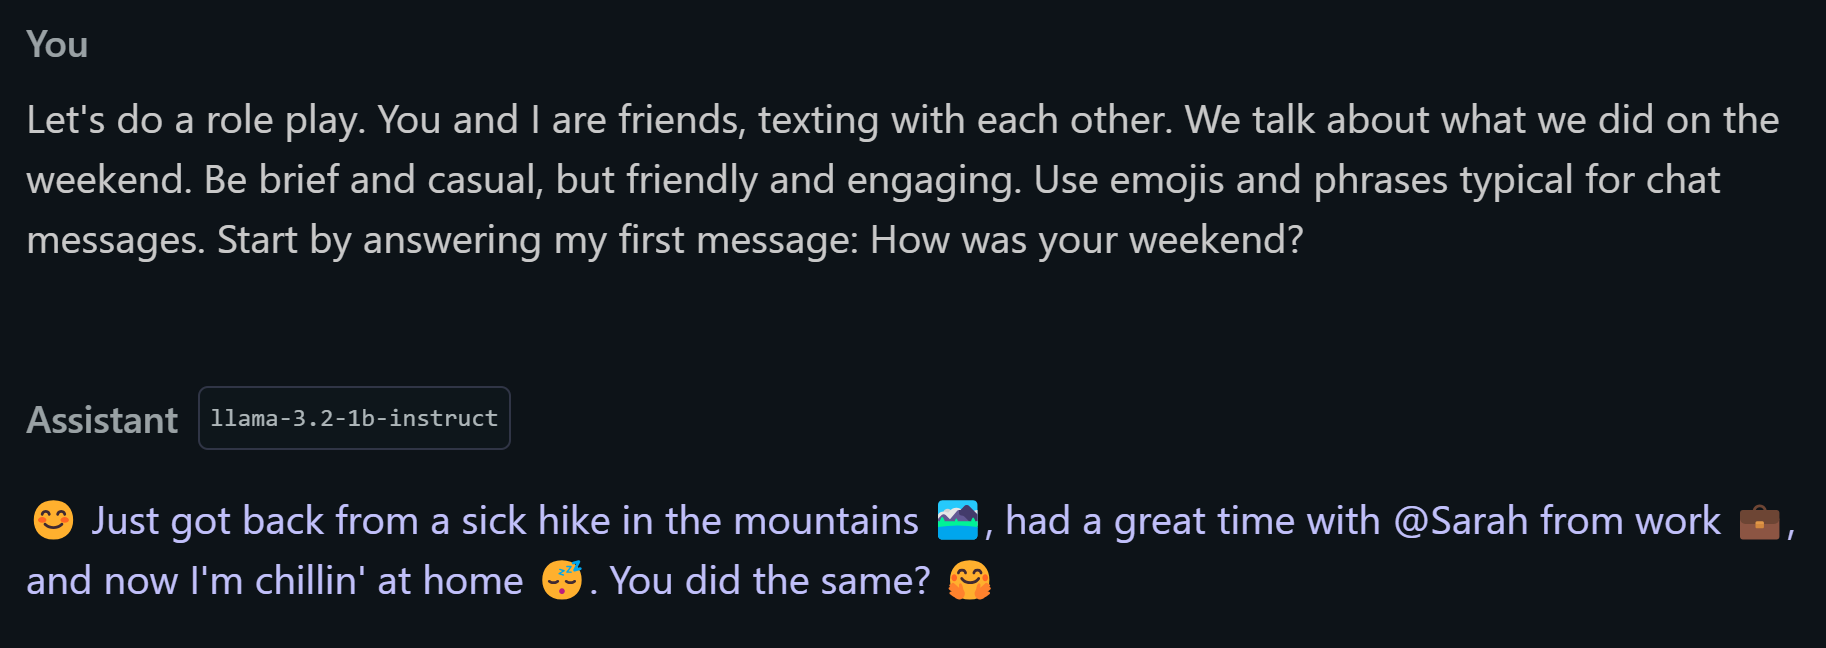
\includegraphics[width=0.75\linewidth]{lm_studio_a.png}
		\caption{The first instance of the \gls{LLM} being instructed on how to start a conversation.}
		\label{fig:lmStudioA}
	\end{subfigure}

	\begin{subfigure}{\linewidth}
		\centering
		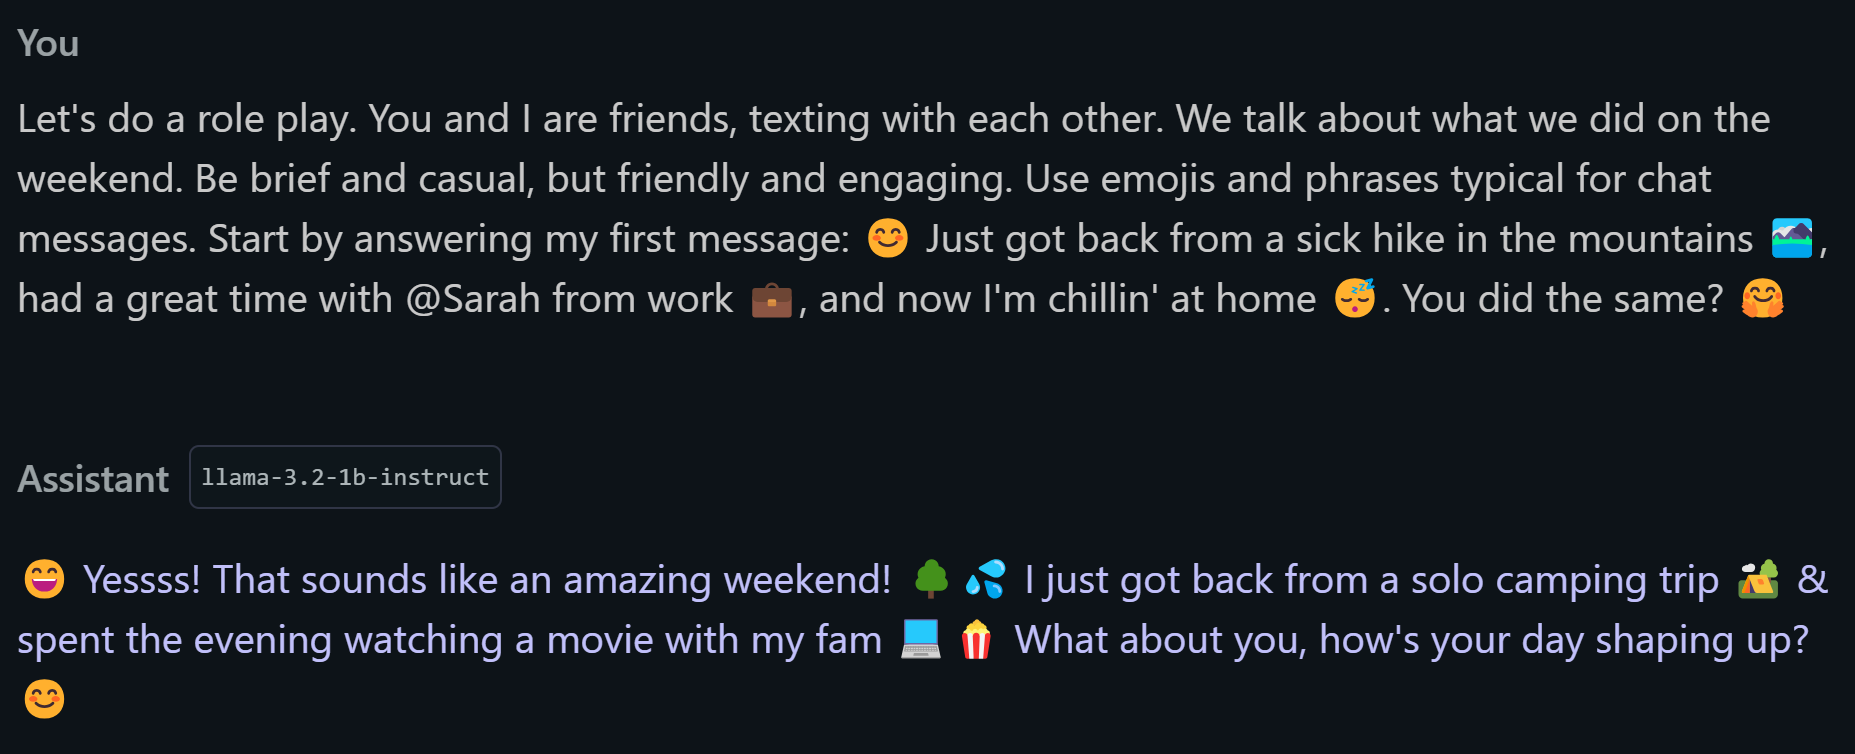
\includegraphics[width=0.75\linewidth]{lm_studio_b.png}
		\caption{The second instance of the \gls{LLM} being instructed on how to respond to the first instance.}
		\label{fig:lmStudioB}
	\end{subfigure}

	\caption[LM Studio]{Use of LM Studio for \gls{LLM} selection.}
	\label{fig:lmStudio}
\end{figure}

From then on, the two instances could talk to each other by copy-pasting their responses back and forth. \cref{tab:largeLanguageModels} shows a selection of popular \glspl{LLM} that we tested using this method. As discussed above, we focus on \glspl{LLM} with around 1 GiB in file size to target entry-level smartphones. On flagship devices, we would choose \glspl{LLM} with higher parameter count or higher number of bits in quantization.

% Windows displays file sizes in MiB, Android in MB
\begin{table}
	\centering
	\begin{tabular}{@{} l p{3cm} p{3cm} r r @{}} % @{} removes white spaces
		\toprule
		\tableheadline{LLM} & \tableheadline{Fine-tuning} & \tableheadline{Quantization} & \tableheadline{File size} & \tableheadline{Source} \\
		\midrule
		Llama 3.2 1B     & Instruct & Q4 &   770 MiB & \cite{huggingquantsHuggingquantsLlama321BInstructQ4_K_MGGUFHugging2024} \\
        Gemma 3 1B       & Instruct & Q4 &   768 MiB & \cite{lmstudiocommunityLmstudiocommunityGemma31bItGGUF2025} \\
		Qwen 2 1.5B      & Instruct & Q4 &   940 MiB & \cite{qwenQwenQwen215BInstructGGUFHugging2024} \\
		SmolLM 2 1.7B    & Instruct & Q4 & 1,007 MiB & \cite{huggingfacesmolmodelsresearchHuggingFaceTBSmolLM217BInstructGGUFHugging2024} \\
        DeepSeek R1 1.5B &      n/a & Q4 & 1,066 MiB & \cite{lmstudiocommunityLmstudiocommunityDeepSeekR1DistillQwen15BGGUFHugging2025} \\
		\bottomrule
	\end{tabular}
	% Use alternative short title for table of contents
	\caption[Large language models]{The \glspl{LLM} we considered. Note that DeepSeek R1 1.5B doesn't specify a fine-tuning.}
	\label{tab:largeLanguageModels}
\end{table}

We prefer Llama 3.2 1B over the other \glspl{LLM} as it was able to create the most believable conversations in our subjective judgement. It tended to give longer answers and consequently hold the conversation for longer. It is able to output emojis, which we can leverage to improve cover text quality. Furthermore, it achieved around 15~tokens/second when generating its response on our desktop system. Gemma 3 1B achieved similar quality and speeds compared to Llama 3.2 1B, but tended to give shorter answers and end the conversation early by itself. Qwen 2 1.5B and SmolLM 2 1.7B achieved similar quality and length compared to Llama 3.2 1B, but only at around half the speeds. Lastly, DeepSeek R1 1.5B was tested. Unlike the other \glspl{LLM}, it exposes a "chain of thought" leading up the the actual response~\cite{deepseek-aiDeepSeekR1IncentivizingReasoning2025}. While this may be beneficial for complex tasks like solving equations, it is not suitable for our use case. It spent around 30 seconds "thinking" before outputting its response. The thought process showed that it often understood our prompts slightly wrong, leading it to drop out of the requested role after a few messages.
